\documentclass[a4paper, 12pt]{article}
\usepackage{maxwell}
\usepackage{tcolorbox}
\title{Maxwell's Distribution}
\author{Murad Bashirov}
\date{}
\begin{document}
\begin{titlepage}
    \maketitle
    \abstract{We will talk about probability theorem and go deep in the Maxwell's distribution, and give  some  problems that I
    found about Maxwell's distribution}
    \tableofcontents
\end{titlepage}
\section{Introduction}
\subsection{Information about Probability}
Assume that we have a system formed  by really high number of particles.
Also assume that our particles characterized by some quantity, which can only have some discrete values:
$$\u_1,\u_2,\ldots,\u_n$$
Let us make a very great number $N$ of measurements of the quantity $\u$, bringing the system before 
each measurement to the same initial state. Instead of performing repeated measurements of the
same system, we can take $N$ identical systems in the same state and measure the quantity 
$\u$ once in all these systems. Such a set of identical systems in an identical state is called a 
\emph{statistical ensemble}.

Let $N_1$ be the measurements that give result $\u_1$ and like so, $N_i$ will be measurements for $x_i$.
This is obvious that $\sum N_i = N$ which is total number of systems that ensemble. So the quantity $\frac{N_i}{N}$ called 
\emph{relative frequency} which shows appearence of resuly $\u_i$, and if we take the so big amount of ensemble systems
that ratio will give us \textbf{probability of appearance} of the result: $$P_i=\lim_{N\to\infty}\frac{N_i}{N}$$
And from here if we take sum of both sides:$$\sum P_i =\sum \lim_{N\to\infty}\frac{N_i}{N}=1$$
since $\sum N_i =N$. With this definition we can also get the information about probability of being in two different quantity, namely:
$$P_{i\text{ or }k}=\frac{N_i+N_k}{N}=P_i+P_k$$

Furthermore assume that particles not only defined by $\u_i$ also there is another quantity $\veps$ also characterizes the particles.
Lets find  the $P(\u_i,\veps_k )$ by the definition $N(\u_i)=P(\u_i)N$ also $\veps$ does not depend on $\u$ so:
$$N(\u_i,\veps_k)=N(\u_i)P(\veps_k)=P(\u_i)NP(\veps_k)$$
So \begin{equation} \label{eq:multiply}
    P(\u_i,\veps_k )=P(\u_i)P(\veps_k)
\end{equation}

We can also find the mean value of some quantity $\u$ with knowing $P(\u)$:
$$\langle \u \rangle =\frac{\sum N_i \u_i}{N}=\sum P(\u_i) \u_i$$
\newpage
\subsection{Probability distribution function}
Let us go further and say that our quantity is not discrete. Here is diagram for simplifying:



% Pattern Info
 
\tikzset{
pattern size/.store in=\mcSize, 
pattern size = 5pt,
pattern thickness/.store in=\mcThickness, 
pattern thickness = 0.3pt,
pattern radius/.store in=\mcRadius, 
pattern radius = 1pt}
\makeatletter
\pgfutil@ifundefined{pgf@pattern@name@_r6fzum5wv}{
\pgfdeclarepatternformonly[\mcThickness,\mcSize]{_r6fzum5wv}
{\pgfqpoint{0pt}{0pt}}
{\pgfpoint{\mcSize+\mcThickness}{\mcSize+\mcThickness}}
{\pgfpoint{\mcSize}{\mcSize}}
{
\pgfsetcolor{\tikz@pattern@color}
\pgfsetlinewidth{\mcThickness}
\pgfpathmoveto{\pgfqpoint{0pt}{0pt}}
\pgfpathlineto{\pgfpoint{\mcSize+\mcThickness}{\mcSize+\mcThickness}}
\pgfusepath{stroke}
}}
\makeatother
\tikzset{every picture/.style={line width=0.75pt}} %set default line width to 0.75pt        
\begin{figure}[h!]
    \centering
    \begin{tikzpicture}[x=0.75pt,y=0.75pt,yscale=-1,xscale=1]
    %uncomment if require: \path (0,308); %set diagram left start at 0, and has height of 308

    %Shape: Rectangle [id:dp8320684478804092] 
    \draw   (168.83,113.33) -- (183.33,113.33) -- (183.33,181) -- (168.83,181) -- cycle ;
    %Shape: Rectangle [id:dp46313903260005507] 
    \draw   (183.33,104.67) -- (198.86,104.67) -- (198.86,181) -- (183.33,181) -- cycle ;
    %Shape: Rectangle [id:dp637544228474491] 
    \draw   (199,90) -- (213.36,90) -- (213.36,181) -- (199,181) -- cycle ;
    %Shape: Rectangle [id:dp9111653973633418] 
    \draw   (154.33,137) -- (168,137) -- (168,181) -- (154.33,181) -- cycle ;
    %Shape: Rectangle [id:dp48371722593765853] 
    \draw   (139.83,154) -- (155,154) -- (155,181) -- (139.83,181) -- cycle ;
    %Shape: Rectangle [id:dp6712731805880472] 
    \draw   (125.33,167) -- (140,167) -- (140,181) -- (125.33,181) -- cycle ;
    %Curve Lines [id:da8724153525294642] 
    \draw  [dash pattern={on 4.5pt off 4.5pt}]  (99,181) .. controls (119.71,188.35) and (170,128.67) .. (209,84.67) .. controls (248,40.67) and (332,134) .. (374,155.67) .. controls (416,177.33) and (432,178.67) .. (516,182.67) ;
    %Straight Lines [id:da6621967085481852] 
    \draw    (99,181) -- (513,182.65) ;
    \draw [shift={(516,182.67)}, rotate = 180.23] [fill={rgb, 255:red, 0; green, 0; blue, 0 }  ][line width=0.08]  [draw opacity=0] (8.93,-4.29) -- (0,0) -- (8.93,4.29) -- cycle    ;
    %Shape: Rectangle [id:dp38156457938657495] 
    \draw   (214,76) -- (227.71,76) -- (227.71,181) -- (214,181) -- cycle ;
    %Shape: Rectangle [id:dp5491197776137533] 
    \draw   (227.71,74) -- (242.07,74) -- (242.07,181) -- (227.71,181) -- cycle ;
    %Shape: Rectangle [id:dp03637882257480052] 
    \draw   (242.07,76) -- (256.43,76) -- (256.43,181) -- (242.07,181) -- cycle ;
    %Shape: Rectangle [id:dp4132386305863096] 
    \draw  [pattern=_r6fzum5wv,pattern size=6pt,pattern thickness=0.75pt,pattern radius=0pt, pattern color={rgb, 255:red, 0; green, 0; blue, 0}] (257,81.67) -- (270.79,81.67) -- (270.79,181) -- (257,181) -- cycle ;
    %Shape: Rectangle [id:dp026924080774506365] 
    \draw   (270.79,88.67) -- (285.93,88.67) -- (285.93,181) -- (270.79,181) -- cycle ;
    %Shape: Rectangle [id:dp8626972827619077] 
    \draw   (286,96.67) -- (300.29,96.67) -- (300.29,181) -- (286,181) -- cycle ;
    %Shape: Rectangle [id:dp8897832831477368] 
    \draw   (300,108.67) -- (314.64,108.67) -- (314.64,181) -- (300,181) -- cycle ;
    %Shape: Rectangle [id:dp9181809288915517] 
    \draw   (315,118.67) -- (329,118.67) -- (329,181) -- (315,181) -- cycle ;
    %Straight Lines [id:da2905135378118493] 
    \draw    (262,111.67) -- (292,62.67) ;

    % Text Node
    \draw (270.97,50.96) node [anchor=north west][inner sep=0.75pt]  [rotate=-337.72]  {$\text{Area}$};
    % Text Node
    \draw (297.67,40.44) node [anchor=north west][inner sep=0.75pt]  [rotate=-337.7]  {$\ =\Delta P$};
    % Text Node
    \draw (244.07,187.4) node [anchor=north west][inner sep=0.75pt]    {$\u$};
    % Text Node
    \draw (272.79,184.4) node [anchor=north west][inner sep=0.75pt]    {$\u+\Delta \u$};
    \end{tikzpicture}
    \caption{Visualation with histogram}
\end{figure}
% Pattern Info
 
\tikzset{
pattern size/.store in=\mcSize, 
pattern size = 5pt,
pattern thickness/.store in=\mcThickness, 
pattern thickness = 0.3pt,
pattern radius/.store in=\mcRadius, 
pattern radius = 1pt}
\makeatletter
\pgfutil@ifundefined{pgf@pattern@name@_1gqfwhjel}{
\pgfdeclarepatternformonly[\mcThickness,\mcSize]{_1gqfwhjel}
{\pgfqpoint{0pt}{0pt}}
{\pgfpoint{\mcSize+\mcThickness}{\mcSize+\mcThickness}}
{\pgfpoint{\mcSize}{\mcSize}}
{
\pgfsetcolor{\tikz@pattern@color}
\pgfsetlinewidth{\mcThickness}
\pgfpathmoveto{\pgfqpoint{0pt}{0pt}}
\pgfpathlineto{\pgfpoint{\mcSize+\mcThickness}{\mcSize+\mcThickness}}
\pgfusepath{stroke}
}}
\makeatother

% Pattern Info
 
\tikzset{
pattern size/.store in=\mcSize, 
pattern size = 5pt,
pattern thickness/.store in=\mcThickness, 
pattern thickness = 0.3pt,
pattern radius/.store in=\mcRadius, 
pattern radius = 1pt}
\makeatletter
\pgfutil@ifundefined{pgf@pattern@name@_w31vr5buc}{
\pgfdeclarepatternformonly[\mcThickness,\mcSize]{_w31vr5buc}
{\pgfqpoint{0pt}{0pt}}
{\pgfpoint{\mcSize+\mcThickness}{\mcSize+\mcThickness}}
{\pgfpoint{\mcSize}{\mcSize}}
{
\pgfsetcolor{\tikz@pattern@color}
\pgfsetlinewidth{\mcThickness}
\pgfpathmoveto{\pgfqpoint{0pt}{0pt}}
\pgfpathlineto{\pgfpoint{\mcSize+\mcThickness}{\mcSize+\mcThickness}}
\pgfusepath{stroke}
}}
\makeatother
\tikzset{every picture/.style={line width=0.75pt}} %set default line width to 0.75pt        
\begin{figure}[h!]
    \centering
    \begin{tikzpicture}[x=0.75pt,y=0.75pt,yscale=-1,xscale=1]
    %uncomment if require: \path (0,308); %set diagram left start at 0, and has height of 308

    %Curve Lines [id:da8724153525294642] 
    \draw    (99,181) .. controls (119.71,188.35) and (169.67,130) .. (209,84.67) .. controls (248.33,39.33) and (332,134) .. (374,155.67) .. controls (416,177.33) and (432,178.67) .. (516,182.67) ;
    %Straight Lines [id:da6621967085481852] 
    \draw    (99,181) -- (513,182.65) ;
    \draw [shift={(516,182.67)}, rotate = 180.23] [fill={rgb, 255:red, 0; green, 0; blue, 0 }  ][line width=0.08]  [draw opacity=0] (8.93,-4.29) -- (0,0) -- (8.93,4.29) -- cycle    ;
    %Straight Lines [id:da18418346383431583] 
    \draw    (99,181) -- (99,27.5) ;
    \draw [shift={(99,24.5)}, rotate = 450] [fill={rgb, 255:red, 0; green, 0; blue, 0 }  ][line width=0.08]  [draw opacity=0] (8.93,-4.29) -- (0,0) -- (8.93,4.29) -- cycle    ;
    %Shape: Rectangle [id:dp6073214185474616] 
    \draw  [color={rgb, 255:red, 0; green, 0; blue, 0 }  ,draw opacity=1 ][pattern=_1gqfwhjel,pattern size=6pt,pattern thickness=0.75pt,pattern radius=0pt, pattern color={rgb, 255:red, 0; green, 0; blue, 0}] (263,84) --  (263,181.57) -- (272,181.57) --(272,84);
    %Shape: Right Triangle [id:dp6223355704316667] 
    \draw  [color={rgb, 255:red, 0; green, 0; blue, 0 }  ,draw opacity=1 ][pattern=_w31vr5buc,pattern size=6pt,pattern thickness=0.75pt,pattern radius=0pt, pattern color={rgb, 255:red, 0; green, 0; blue, 0}] (272,84) -- (263,79.33) --  (263,84);
    %straight line
    \draw    (265,111.67) -- (292,62.67) ;
    % Text Node
    \draw (270.97,50.96) node [anchor=north west][inner sep=0.75pt]  [rotate=-337.72]  {$\text{Area}$};
    % Text Node
    \draw (297.67,40.44) node [anchor=north west][inner sep=0.75pt]  [rotate=-337.7]  {$\ =\mathrm{d} P$};
    % Text Node
    \draw (249,188.4) node [anchor=north west][inner sep=0.75pt]    {$\u$};
    % Text Node
    \draw (272.79,184.4) node [anchor=north west][inner sep=0.75pt]    {$\u+\mathrm{d} \u$};
    %Text Node
    \draw (65, 30) node [anchor=north west][inner sep=0.75pt]  {$f(\u)$};
    \end{tikzpicture}
    \caption{Visualation with graph}
\end{figure}


The histogram characterizes graphically the probability of obtaining
results of measurements confined within different intervals of width $\Delta \u$. If we take the limit $\Delta \u \to 0$ we will
get those histogram transforms to smooth curve.The function $f(\u)$ defining this curve 
analytically is called a \emph{probability distribution function}.

In accordance with the procedure followed in plotting the distribution
curve, the area of the bar of width $\dd \u$ equals the probability of the fact that the result of a
measurement will be within the range from $\u$ to $u + \dd\u$. Denoting this probability by $\dd P$ 
we can write that $$\dd P(\u) = f(\u)\dd\u$$
So integrating both sides we see that $$\int f(\u)\dd\u=1$$ Knowing the $f(\u)$ we can find the mean values:
$$\langle \u \rangle=\int \u \dd P=\int \u f(\u)\dd\u$$ Or with the similar method we can find mean value of any function $g(\u)$
$$\langle g(\u)\rangle =\int g(\u)f(\u)\dd u$$
\section{The Maxwell's Distribution}\label{sec:maxwell}
\subsection{Proving the Maxwell's Distribution}
We shall use the following procedure to find a way of quantitatively describing the distribution of 
molecules by velocity magnitudes. Let us take Cartesian coordinate axes in an imaginary space which
we shall call $v$-space (velocity space). We shall lay off the values of $v_x, v_y, v_z$ of individual 
molecules along these axes (what we have in view are the velocity components along the axes $x, y, z$ taken
in conventional space). Hence, a point in this $v$-space will correspond to the velocity of each molecule.
Owing to collisions, the positions of the points will continuously change, but their density at each 
place will remain unchanged (we are dealing with equlibrium state).


\tikzset{every picture/.style={line width=0.75pt}} %set default line width to 0.75pt        
\begin{figure}[h!]
    \centering
    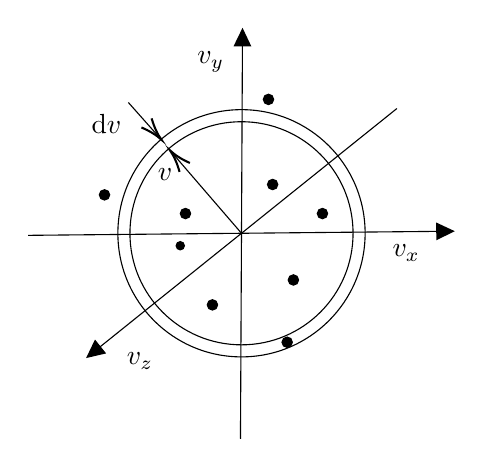
\begin{tikzpicture}[x=0.75pt,y=0.75pt,yscale=-1,xscale=1]
    %uncomment if require: \path (0,308); %set diagram left start at 0, and has height of 308

    %Straight Lines [id:da49644144765049947] 
    \draw    (330.98,60.5) -- (330,255.5) ;
    \draw [shift={(331,57.5)}, rotate = 90.29] [fill={rgb, 255:red, 0; green, 0; blue, 0 }  ][line width=0.08]  [draw opacity=0] (8.93,-4.29) -- (0,0) -- (8.93,4.29) -- cycle    ;
    %Straight Lines [id:da4067851869894472] 
    \draw    (227.75,157.5) -- (430.25,155.53) ;
    \draw [shift={(433.25,155.5)}, rotate = 539.44] [fill={rgb, 255:red, 0; green, 0; blue, 0 }  ][line width=0.08]  [draw opacity=0] (8.93,-4.29) -- (0,0) -- (8.93,4.29) -- cycle    ;
    %Straight Lines [id:da17969570301166127] 
    \draw    (257.96,214.75) -- (405.38,96.38) ;
    \draw [shift={(255.63,216.63)}, rotate = 321.24] [fill={rgb, 255:red, 0; green, 0; blue, 0 }  ][line width=0.08]  [draw opacity=0] (8.93,-4.29) -- (0,0) -- (8.93,4.29) -- cycle    ;
    %Shape: Circle [id:dp2978843034346139] 
    \draw   (276.75,156.5) .. controls (276.75,126.81) and (300.81,102.75) .. (330.5,102.75) .. controls (360.19,102.75) and (384.25,126.81) .. (384.25,156.5) .. controls (384.25,186.19) and (360.19,210.25) .. (330.5,210.25) .. controls (300.81,210.25) and (276.75,186.19) .. (276.75,156.5) -- cycle ;
    %Shape: Circle [id:dp5964721573198295] 
    \draw   (270.94,156.5) .. controls (270.94,123.6) and (297.6,96.94) .. (330.5,96.94) .. controls (363.4,96.94) and (390.06,123.6) .. (390.06,156.5) .. controls (390.06,189.4) and (363.4,216.06) .. (330.5,216.06) .. controls (297.6,216.06) and (270.94,189.4) .. (270.94,156.5) -- cycle ;
    %Straight Lines [id:da45406047896510526] 
    \draw    (330.5,156.5) -- (302.81,124.39) -- (297.31,118.01) ;
    \draw [shift={(296,116.5)}, rotate = 409.22] [color={rgb, 255:red, 0; green, 0; blue, 0 }  ][line width=0.75]    (10.93,-3.29) .. controls (6.95,-1.4) and (3.31,-0.3) .. (0,0) .. controls (3.31,0.3) and (6.95,1.4) .. (10.93,3.29)   ;
    %Straight Lines [id:da2439720548719735] 
    \draw    (276,93.5) -- (290.67,110.01) ;
    \draw [shift={(292,111.5)}, rotate = 228.37] [color={rgb, 255:red, 0; green, 0; blue, 0 }  ][line width=0.75]    (10.93,-3.29) .. controls (6.95,-1.4) and (3.31,-0.3) .. (0,0) .. controls (3.31,0.3) and (6.95,1.4) .. (10.93,3.29)   ;
    %Shape: Circle [id:dp40423032474491927] 
    \draw  [fill={rgb, 255:red, 0; green, 0; blue, 0 }  ,fill opacity=1 ] (343,133) .. controls (343,131.62) and (344.12,130.5) .. (345.5,130.5) .. controls (346.88,130.5) and (348,131.62) .. (348,133) .. controls (348,134.38) and (346.88,135.5) .. (345.5,135.5) .. controls (344.12,135.5) and (343,134.38) .. (343,133) -- cycle ;
    %Shape: Circle [id:dp9303065616806931] 
    \draw  [fill={rgb, 255:red, 0; green, 0; blue, 0 }  ,fill opacity=1 ] (301,147) .. controls (301,145.62) and (302.12,144.5) .. (303.5,144.5) .. controls (304.88,144.5) and (306,145.62) .. (306,147) .. controls (306,148.38) and (304.88,149.5) .. (303.5,149.5) .. controls (302.12,149.5) and (301,148.38) .. (301,147) -- cycle ;
    %Shape: Circle [id:dp4846243689306988] 
    \draw  [fill={rgb, 255:red, 0; green, 0; blue, 0 }  ,fill opacity=1 ] (299,162.5) .. controls (299,161.4) and (299.9,160.5) .. (301,160.5) .. controls (302.1,160.5) and (303,161.4) .. (303,162.5) .. controls (303,163.6) and (302.1,164.5) .. (301,164.5) .. controls (299.9,164.5) and (299,163.6) .. (299,162.5) -- cycle ;
    %Shape: Circle [id:dp6466212282995909] 
    \draw  [fill={rgb, 255:red, 0; green, 0; blue, 0 }  ,fill opacity=1 ] (353,179) .. controls (353,177.62) and (354.12,176.5) .. (355.5,176.5) .. controls (356.88,176.5) and (358,177.62) .. (358,179) .. controls (358,180.38) and (356.88,181.5) .. (355.5,181.5) .. controls (354.12,181.5) and (353,180.38) .. (353,179) -- cycle ;
    %Shape: Circle [id:dp8971905699129288] 
    \draw  [fill={rgb, 255:red, 0; green, 0; blue, 0 }  ,fill opacity=1 ] (314,191) .. controls (314,189.62) and (315.12,188.5) .. (316.5,188.5) .. controls (317.88,188.5) and (319,189.62) .. (319,191) .. controls (319,192.38) and (317.88,193.5) .. (316.5,193.5) .. controls (315.12,193.5) and (314,192.38) .. (314,191) -- cycle ;
    %Shape: Circle [id:dp1504932565119863] 
    \draw  [fill={rgb, 255:red, 0; green, 0; blue, 0 }  ,fill opacity=1 ] (341,92) .. controls (341,90.62) and (342.12,89.5) .. (343.5,89.5) .. controls (344.88,89.5) and (346,90.62) .. (346,92) .. controls (346,93.38) and (344.88,94.5) .. (343.5,94.5) .. controls (342.12,94.5) and (341,93.38) .. (341,92) -- cycle ;
    %Shape: Circle [id:dp5069336937258984] 
    \draw  [fill={rgb, 255:red, 0; green, 0; blue, 0 }  ,fill opacity=1 ] (262,138) .. controls (262,136.62) and (263.12,135.5) .. (264.5,135.5) .. controls (265.88,135.5) and (267,136.62) .. (267,138) .. controls (267,139.38) and (265.88,140.5) .. (264.5,140.5) .. controls (263.12,140.5) and (262,139.38) .. (262,138) -- cycle ;
    %Shape: Circle [id:dp11972303219299696] 
    \draw  [fill={rgb, 255:red, 0; green, 0; blue, 0 }  ,fill opacity=1 ] (350,209) .. controls (350,207.62) and (351.12,206.5) .. (352.5,206.5) .. controls (353.88,206.5) and (355,207.62) .. (355,209) .. controls (355,210.38) and (353.88,211.5) .. (352.5,211.5) .. controls (351.12,211.5) and (350,210.38) .. (350,209) -- cycle ;
    %Shape: Circle [id:dp20783273065922692] 
    \draw  [fill={rgb, 255:red, 0; green, 0; blue, 0 }  ,fill opacity=1 ] (367,147) .. controls (367,145.62) and (368.12,144.5) .. (369.5,144.5) .. controls (370.88,144.5) and (372,145.62) .. (372,147) .. controls (372,148.38) and (370.88,149.5) .. (369.5,149.5) .. controls (368.12,149.5) and (367,148.38) .. (367,147) -- cycle ;

    % Text Node
    \draw (289,123.9) node [anchor=north west][inner sep=0.75pt]    {$v$};
    % Text Node
    \draw (257,97.9) node [anchor=north west][inner sep=0.75pt]    {$\mathrm{d} v$};
    % Text Node
    \draw (402,160.9) node [anchor=north west][inner sep=0.75pt]    {$v_{x}$};
    % Text Node
    \draw (308,67.9) node [anchor=north west][inner sep=0.75pt]    {$v_{y}$};
    % Text Node
    \draw (274,212.9) node [anchor=north west][inner sep=0.75pt]    {$v_{z}$};


    \end{tikzpicture}
    \caption{$v$-space}
\end{figure}
Owing to all the directions of motion having equal rights, the arrangement of the points relative to the 
origin of coordinates will be spherically symmetrical. Hence, the density of the points in
our $v$-space can depend only on the magnitude of the velocity $v$. Let us denote this density by 
$Nf(v)$ (here $N$ is the total number of molecules in the given mass of gas). Hence, the number of
molecules whose velocity components are within the limits from $v_x \text{ to } v_x + \dd v_x$, from 
$v_y \text{ to } v_y +\dd v_y$ , and from $v_z \text{ to } v_z + \dd v_z$ can be written in the form
\begin{equation} \label{eq:probvxvyvz}
    \dd N_{v_x,v_y,v_z} =Nf(v)\dd v_x\dd v_y\dd v_z
\end{equation}
The product of three small changes gives ann element of volume in $v$-space.

So from the volume of the element in $v$-space the equation simplifies:
\begin{equation}
    \label{eq:main}
    \dd N_v=Nf(v)4\pi v^2\dd v
\end{equation}

the probability of the velocity component $v_x$ of a molecule having a value within the limits from $v_x \text{ to }
v_x + \dd v_x$ can be written in the form
$$\dd P_{v_x} = \phi(v_x) \dd v_x$$ where $\phi$ is distribution function. For the other components the equations will 
symmetrical. So by the equation \ref{eq:multiply}: $$\dd P_{v_x,v_y,v_z}=\phi(v_x)\phi(v_y)\phi(v_z)\dd v_x\dd v_y\dd v_z$$
Also taking into account equation \ref{eq:probvxvyvz} we get that:
\begin{equation} \label{eq:fvvxvyvz}
    f(v)=\phi(v_x)\phi(v_y)\phi(v_z)
\end{equation} So if we take logarithm both sides :$$\ln f(v)=\ln \phi(v_x)+\ln \phi(v_y)+\ln\phi(v_z)
$$ differentiating this equation with respect to $v_x$:
\begin{equation} \label{eq:parderf}
    \frac{f'(v)}{f(v)}\pdv{v}{v_x}=\frac{\phi'(v_x)}{\phi(v_x)}
\end{equation} 
Since $v=\sqrt{v_x^2+v_y^2+v_z^2}$ we can take partial derivative
$$\pdv{v}{v_x}=\frac{v_x}{\sqrt{v_x^2+v_y^2+v_z^2}}=\frac{v_x}{v}$$
Plugging this in equation \ref{eq:parderf}:
$$\frac{f'(v)}{f(v)}\frac{1}{v}=\frac{\phi'(v_x)}{\phi(v_x)}\frac{1}{v_x}$$
Since right hand side is not dependent on $v_y$ and $v_z$(also left hand side too, it is an equality). Consequently it cannot depend on $v_x$ too
because they are symmetrical in definition of $f(v)$, namely equation \ref{eq:fvvxvyvz}.So that equation is equal to constant.
Let that constant be $-\alpha$(why negative, it can be positive but at the end you will see it becames negative)
So: $$\frac{\phi'(v_x)}{\phi(v_x)}=-\alpha v_x$$ Integrating both sides: $$\phi(v_x))=C\exp(-\frac{\alpha v_x^2}{2})$$
For $v_y$ and $v_z$ equations will be symmetrical. Thus by the equation \ref{eq:fvvxvyvz}:
$$f(v)=C^3\exp(-\frac{\alpha(v_x^2+v_y^2+v_z^2)}{2})=C^3e^{-\frac{\alpha v^2}{2}}$$
We can find constant $C$ from normalization of $\phi$(note that $v_x$ can be any real number):
\begin{equation}\label{eq:normal}
    C\int_{-\infty}^\infty \exp(-\frac{\alpha v_x^2}{2})\dd v_x=1
\end{equation} 
We can substitute new variable and change this to Gaussian integral. So at the end we get $$C=\sqrt{\frac{\alpha}{2\pi}}$$
So our distribution functions:
\begin{align}
    \label{eq:compphi}
    \phi(v_x)&=\sqrt{\frac{\alpha}{2\pi}}\exp(-\frac{\alpha v_x^2}{2}) \\
    \label{eq:compf}
    f(v)&=\qty(\frac{\alpha}{2\pi})^{3/2}\exp(-\frac{\alpha v^2}{2}) 
\end{align}
To find constant $\alpha$ we will calculate the value of $\langle v_x^2\rangle$ with using equation \ref{eq:compphi} and knowing that
it's equal  to $\frac{kT}{m}$ according to \textbf{Lemma} \ref{lem:1}. So:
\begin{equation}\label{eq:normalvx}
    \langle v_x^2\rangle=\int_{-\infty}^\infty v_x^2\phi(v_x)\dd v_x=\sqrt{\frac{\alpha}{2\pi}}\int_{-\infty}^\infty v_x^2\exp(-\frac{\alpha v_x^2}{2})\dd v_x
\end{equation}
And this can be done with integration by parts and Gaussian integral. So overall we get:
$$\langle v_x^2\rangle=\frac{1}{\alpha}\implies\alpha=\frac{m}{kT}$$

So finally we show that $$f(v)=\qty(\frac{m}{2\pi kT})^{\frac{3}{2}}\exp(-\frac{mv^2}{2kT})$$
But if we want to find the actual probability distribution function, we have to multiply it by $4\pi v^2$ because of equation \ref{eq:main}

So overall:
\\

\hskip 2in \boxed{$$F(v)=4\pi v^2\qty(\frac{m}{2\pi kT})^{\frac{3}{2}}\exp(-\frac{mv^2}{2kT})$$}\hfill $\blacksquare$

\begin{lemma}\label{lem:1}
    In the ideal gases the mean square of the one of the components of the velocity is equals to $\frac{kT}{m}$
\end{lemma}
\begin{proof}     
    We need to relate pressure to energy so that we can get equation for root mean square
    velocity. Consider this scenario

    \begin{figure}[h!]
        \centering
        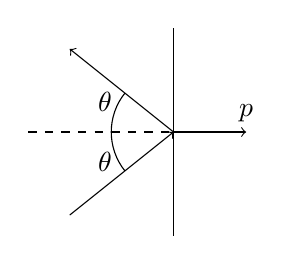
\begin{tikzpicture}[x=0.75pt,y=0.75pt,yscale=-1,xscale=1]
            \coordinate (O) at (200,100);
            \draw (200,50) -- (200,150);
            \draw[->] (150,140) -- (200,100);
            \draw[->] (200,100) -- (150,60);
            \draw[dashed] (130,100) -- (200,100);
            \draw[->] (200,100) -- (235,100) node[above]{$p$};
            \draw (176.58,81.26) arc (218.66:141.3402:30);
            \draw (175,95) node[anchor=south east]{$\theta$};
            \draw (175,105) node[anchor=north east]{$\theta$};
        \end{tikzpicture}
        \caption{Molecule collides with the wall}
        \label{fig:elasticcol}
    \end{figure}

    So the momentum change is $$\dd p=2mv\cos\theta \dd n=\dd N\frac{\dd \Omega}{4\pi}\frac{2mv^2\cos^2\theta\Delta S\Delta t}{V}$$
    If we substitute formula for $\dd \Omega$ and integrate it we get $$\dd p=\dd N\frac{2mv^2 \Delta S\Delta t}{2\pi V}\underbrace{\int_0^{\pi/2}\cos^2\theta\sin\theta\dd\theta}_{1/3} \underbrace{\int_0^{2\pi}\dd \phi}_{2\pi}$$
    So overall $$\dd p=\dd N \frac{mv^2 \Delta S\Delta t}{3V}$$Once again integrating this expression we get total momentum change in area $\Delta S$ with time $\Delta t$
    $$\Delta p=\frac{m\Delta S\Delta t}{3V}\int_{0}^{\infty}v^2\dd N$$
    The expression $\frac{1}{N}\int_{0}^{\infty}v^2\dd N$ is the mean value of square velocity. So substituting this yields
    $$\Delta p=\frac{m\Delta S\Delta t}{3V}N\langle v^2\rangle=\frac{1}{3}nm\langle v^2\rangle\Delta S\Delta t$$
    where $n$ is molecules per volume. This is momentum change. So if we divide it by $\Delta t$ we will get  force, and again dividing by $\Delta S$ we will get the pressure.So
    $$P = \frac{1}{3}nm\langle v^2\rangle=\frac{2}{3}n\left<\frac{mv^2}{2}\right>=\frac{2}{3}m\langle \veps \rangle$$
    And if we compare this result with the ideal gas law we can see that $$\langle \veps \rangle=\frac{3}{2}kT$$
    And by the definition of kinetic energy $$\langle v^2\rangle=\frac{3kT}{m}$$ Also the velocity has components: $\langle v^2\rangle = \langle v_x^2\rangle+\langle v_y^2\rangle+\langle v_z^2\rangle$
    . In this equation all three components has equal rights, so they have to be equal. Overall we get that $$\langle v_x^2\rangle=\frac{kT}{m}$$
\end{proof}

\subsection{Applying Maxwell's Distribution}
We have the probability distribution function, so we can find some values like mean velocity or most probable velocity.\\
For finding mean velocity $\langle v\rangle$ we  need to integrate:
\begin{equation}\label{eq:meanv}
    \int_0^\infty  v^2F(v)\dd v=4\pi \qty(\frac{m}{2\pi kT})^{\frac{3}{2}}\int_0^\infty\exp(-\frac{mv^2}{2kT})v^3\dd v
\end{equation}
So we can integrate this with substitution and integration by parts.We get:
$$\langle v\rangle=\sqrt{\frac{8kT}{\pi m}}$$

With the same method we can also find $\langle v^2 \rangle$. So integrating:
$$\langle v^2 \rangle=\int_0^\infty v^2 F(v)\dd v=\frac{3kT}{m}$$
And the root of this velocity is called root mean square velocity:$$v_{rms}=\sqrt{\frac{3kT}{m}}$$

For the most probable velocity we need to find the maximum of the $F(v)$, which can be found by taking derivative and setting equal to zero:
$$\exp(-\frac{mv^2}{2kT})\qty(2-\frac{mv^2}{kT})=0$$ From here it is obvious that $$v_{mp}=\sqrt{\frac{2kT}{m}}$$

\newpage
\subsection{Maxwell's Distribution in spherical coordinates}
We can even go further and write Maxwell's distribution not only for a sphere shell but also a tiny element on the system. It is more convenient to use 
spherical coordinates in our $v$-space. Changing from cartesian to spherical:
\tdplotsetmaincoords{60}{110}
%
\pgfmathsetmacro{\rvec}{.8}
\pgfmathsetmacro{\thetavec}{30}
\pgfmathsetmacro{\phivec}{60}
%
\begin{figure}[h!]
    \centering
    \begin{tikzpicture}[scale=5,tdplot_main_coords]
        \coordinate (O) at (0,0,0);
        \draw[thick,->] (0,0,0) -- (1,0,0) node[anchor=north east]{$x$};
        \draw[thick,->] (0,0,0) -- (0,1,0) node[anchor=north west]{$y$};
    \draw[thick,->] (0,0,0) -- (0,0,1) node[anchor=south]{$z$};
        \tdplotsetcoord{P}{\rvec}{\thetavec}{\phivec}
        \draw[color=red,->] (O) -- (P) node[above right] {$P$};
        \node (r) at (0.125,0.21651,0.5){$r$};
        \draw[dashed, color=red] (O) -- (Pxy);
        \draw[dashed] (P) -- (Pxy);
        \draw[dashed] (Pxy) -- (Px) node[left]{$x_P$};
        \draw[dashed] (Pxy) -- (Py) node[above right]{$y_P$};
        \draw[dashed] (P) -- (Pz) node[above left]{$z_P$};
        \tdplotdrawarc{(O)}{0.2}{0}{\phivec}{anchor=north}{$\varphi$}
        \tdplotsetthetaplanecoords{\phivec}
        \tdplotdrawarc[tdplot_rotated_coords]{(0,0,0)}{0.2}{0}%
            {\thetavec}{anchor=south}{$\theta$}
    \end{tikzpicture}
    \caption{Spherical coordinate system}
\end{figure}

The little volume in the cartesian coordinates is $\dd V=\dd x\dd y\dd z$ But we want to simplify things so from basic
trigonometry it is obvious that $$x_P r\sin\theta\cos\varphi\quad y_P=r\sin\theta\sin\varphi\quad z_P=r\cos\theta$$ 
So tiny volume in the spherical coordinates is $$\dd V=r^2\sin\theta\dd\theta\dd r\dd\varphi$$
So Maxwell's distribution changes into(in our $v$-space $r=v$):
$$f(v)=v^2\qty(\frac{m}{2\pi kT})^{\frac{3}{2}}\exp(-\frac{mv^2}{2kT})\sin\theta\dd\theta\dd\varphi$$
So we can use this when averaging things, due to coordinates.
\newpage
\section{Problems}
\subsection{Easy problems}
\begin{problem}
    Do the integrals which was provided in the Section~\ref{sec:maxwell}
\end{problem}

From now on you can use following integrals:
\begin{align}
    \label{eq:int0}
    I_0=\int_0^\infty e^{-ax^2}=\frac12\sqrt{\frac{\pi}{a}}\\
    \label{eq:int1}
    I_1=\int_0^\infty xe^{-ax^2}=\frac{1}{2a}\\
    \label{eq:int2}
    I_2=\int_0^\infty x^2e^{-ax^2}=\frac{1}{4}\sqrt{\frac{\pi}{a^3}}\\
    \label{eq:int3}
    I_3=\int_0^\infty x^3e^{-ax^2}=\frac{1}{2a^2}\\
    \label{eq:int4}
    I_4=\int_0^\infty x^4e^{-ax^2}=\frac{3}{8}\sqrt{\frac{\pi}{a^5}}\\
    \label{eq:int5}
    I_5=\int_0^\infty x^5e^{-ax^2}=\frac{1}{a^3}
\end{align}
\begin{problem}
    Show that for any ideal gas the product of mean velocity and mean inverse velocity is:
    $$\langle v\rangle\left<\frac{1}{v}\right> =\frac{4}{\pi}$$
\end{problem}
\begin{problem}
    Get the formula for Maxwell's distribution in terms of kinetic energy $E$:
    $$F(E)\dd E = a E^{b}\exp(-\frac{E}{kT})\dd E$$
    i.e find the constants $a, b$
\end{problem}
\begin{problem}
    We can also define the distribution in term  of deBroglie wavelength:
    $$\lambda=\frac{h}{mv}$$
    where $h$ is Planck constant. So find the distribution $F(\lambda)\dd\lambda$ in terms of $\lambda$
    $$F(\lambda)\dd\lambda=a\lambda^{-b}\exp(-\frac{c}{\lambda^2})\dd \lambda$$
    i.e find constants $a,b,c$
\end{problem}

\subsection{Intermediate problems}
\begin{problem}
    One mole of ideal gas kept in the vessel. Temperature of the gas is kept constant equal to $T$.
    Gas concentration in the vessel is $n$. Estimate the number of molecules $N_c$ colliging with the flat wall of
    container per unit area $S$ during period of time $\Delta t$ 

    \emph{Hint: first try a simplified problem then generilaze}
\end{problem}
\begin{problem}
    Using Maxwell's distribution calculate pressure of $P$ of ideal gas with concentration $n$ and temperature $T$
\end{problem}

\subsection{Harder problems}
\begin{problem}
    An ideal monoatomic gas is leaking from thermally insulated vessel into vacuum through a tiny hole
    ,which is much smaller than mean free path of gas.\\
    Assuming Maxwell's velocity distribution for the atoms, calculate parameter $\gamma$. which is ratio 
    between average kinetic energy of molecules of gas outside the vessel to average energy oh the gas inside the 
    vessel: $$\gamma=\frac{\langle E_{\text{outside}}\rangle}{\langle E_{\text{inside}}\rangle}$$
    There is no flow back of atoms
\end{problem}
\begin{problem}
    A thermally insulated vessel with thin walls  has a small hole at one of its sides. This vessel was initially empty at the vacuum.
    A thin beam of molecules moving with equal velocities $v_0$  is directed at the hole of the vessel
    in a direction perpendicular to the surface of the hole.
    (arrows show gas molecules)
    \begin{center}
        \tikzset{every picture/.style={line width=0.75pt}} 
        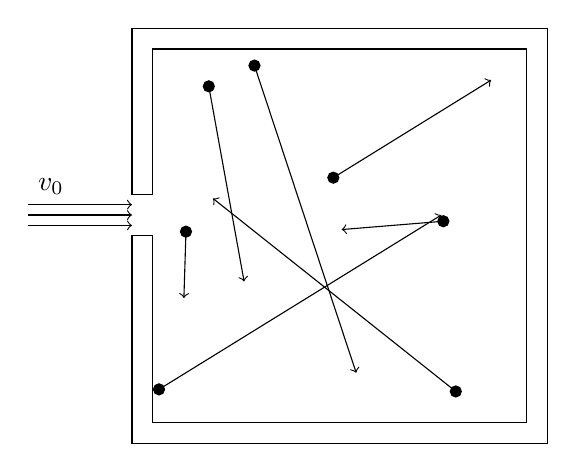
\begin{tikzpicture}[x=0.75pt,y=0.75pt,yscale=-1,xscale=1]
            \draw (100,100) -- (100,20) -- (300,20) -- (300,220) -- (100,220) -- (100,120) -- (110,120) -- (110,210) -- (290,210) -- (290,30) -- (110,30) -- (110,100) -- cycle;
            \draw[<-] (100,105) -- (50,105) node[above right]{$v_0$};
            \draw[->] (50,110) -- (100,110);
            \draw[->] (50,115) -- (100,115);
            \filldraw[black] (159,38) circle (2pt);
            \draw[->] (159,38) -- (208,186);
            \filldraw[black] (250,113) circle (2pt);
            \draw[->] (250,113) -- (201,117);
            \filldraw[black] (137,48) circle (2pt);
            \draw[->] (137,48) -- (154,142);
            \filldraw[black] (113,194) circle (2pt);
            \draw[->] (113,194) -- (249,110);
            \filldraw[black] (256,195) circle (2pt);
            \draw[->] (256,195) -- (139,102);
            \filldraw[black] (126,118) circle (2pt);
            \draw[->] (126,118) -- (125,150);
            \filldraw[black] (197,92) circle (2pt);
            \draw[->] (197,92) -- (273,45);
        \end{tikzpicture}
    \end{center}
    Determine the temperature of the gas $T$ inside the vessel after a long period of time. Molar mass of atoms is $\mu$
\end{problem}
\subsection{Hardest Problems}
Try these problems:
\begin{itemize}
    \item 2020 OPhO Invitational Round Problem 7
    \item 2002 APhO Problem 3
    \item 2015 APhO Problem 2(b)
    \item 2019 APhO Problem 2B
\end{itemize}
\section{Solutions}
\begin{sol}
    \begin{enumerate}
        \item So first integral is equation~\ref{eq:normal}. To do that we just need to substitute $u^2=\frac{\alpha v^2}{2}$ and $\dd u=\dd v\sqrt{\frac{\alpha}{2}}$. So integral becomes
        $$C\sqrt{\frac{2}{\alpha}} \int_{-\infty}^{\infty}e^{-u^2}\dd u=1.$$ And this is Gaussian integral which is equals to $\sqrt{\pi}$. So constant is
        $$\sqrt{\frac{\alpha}{2\pi}}$$
        \item Second integral is equation~\ref{eq:normalvx}.$$\langle v^2\rangle =\sqrt{\frac{\alpha}{2\pi}}\int_{-\infty}^\infty v_x^2\exp(-\frac{\alpha v_x^2}{2})\dd v_x$$
        This can be doable using integration by parts. So we want to differentiate $v_x$ and integrate other part
        \begin{center}
            \begin{tabular}{ c c c }
                & D & I\\ 
                $+$ & $v_x$& $v_xe^{-\frac{\alpha v_x^2}{2}}$\\
                $-$ & $1$ & $-\frac{1}{\alpha}e^{-\frac{\alpha v_x^2}{2}}$
            \end{tabular}
        \end{center}
        So integral becomes $$-\frac{v_x}{2\alpha}e^{-\frac{\alpha v_x^2}{2}}\eval_{-\infty}^\infty+\frac{1}{2\alpha}\int_{-\infty}^\infty e^{-\frac{\alpha v_x^2}{2}}\dd v_x$$
        First term vanishes because of exponential. Second term is same as integral 1. So overall doing same steps we get
        $$\langle v_x^2\rangle=\sqrt{\frac{\alpha}{2\pi}}\sqrt{\frac{2\pi}{\alpha^3}}=\frac{1}{\alpha} $$
        \item Third integral is equation~\ref{eq:meanv}. We can use same method for this.but this time we will different $v^2$.
        So 
        \begin{center}
            \begin{tabular}{ c c c }
                & D & I\\
                $+$&$v^2$& $v\exp(-\frac{mv^2}{2kT})$\\
                $-$&$2v$&$-\frac{kT}{m}\exp(-\frac{mv^2}{2kT})$
            \end{tabular}
        \end{center}
        The same as integral two first term vanishes because of exponential and we left with
        $$\int_0^\infty\frac{kT}{m}2v\exp(-\frac{mv^2}{kT})\dd v$$
        So if we substitute $u=\frac{mv^2}{kT}$ we get $\int_0^\infty2\qty(\frac{kT}{m})^2e^{-u}\dd u=2\qty(\frac{kT}{m})^2$
        Overall $$\langle v\rangle=4\pi \qty(\frac{m}{2\pi kT})^{\frac{3}{2}}2\qty(\frac{kT}{m})^2=\sqrt{\frac{8kT}{\pi m}}$$
    \end{enumerate}
\end{sol}
\begin{sol}
    For this problem we just need to find $\left<\frac{1}{v}\right>$ So by the definition
    $$\left<\frac{1}{v}\right>=\int_0^\infty\frac{f(v)}{v}\dd v=4\pi\qty(\frac{m}{2\pi kT})^{\frac{3}{2}}\int_0^\infty v\exp(-\frac{mv^2}{2kT})\dd v$$
    using provided integral \ref{eq:int1} we get that $$\left<\frac{1}{v}\right>=4\pi\qty(\frac{m}{2\pi kT})^{\frac{3}{2}}\frac{kT}{m}=\sqrt{\frac{2m}{\pi kT}}$$
    And $\langle v \rangle=\sqrt{\frac{8kT}{\pi m}}$ is known so if we multiply them we get $\frac{4}{\pi}$
\end{sol}
\begin{sol}
    Original Maxwell's distribution is 
    $$f(v)\dd v=4\pi v^2\qty(\frac{m}{2\pi kT})^{\frac{3}{2}}\exp(-\frac{mv^2}{2kT})\dd v$$
    For transformation we must have $$F(E)\dd E=f(v)\dd v\implies F(E)\dd E=f(v)\frac{\dd v}{\dd E}\dd E$$
    We can find its derivative by the definition $E=\frac{mv^2}{2}\implies \dv{E}{v}=mv$ So $F(E)\dd E$ is
    \begin{align*}&F(E)\dd E=4\pi v^2\qty(\frac{m}{2\pi kT})^{\frac{3}{2}}\exp(-\frac{mv^2}{2kT})\qty(\frac{1}{mv})\dd E=\\
    &=\frac{2}{\sqrt{\pi}(kT)^{3/2}}\sqrt{E}\exp(-\frac{E}{kT})\dd E\end{align*}
    Or $$a=\frac{2}{\sqrt{\pi}(kT)^{3/2}}\quad b=\frac12$$
\end{sol}
\begin{sol}
    New deBroglie wavelength distribution should satisfy the condition
    $$f(v)\dd v=-F(\lambda)\dd \lambda\implies -f(v)\dv{v}{\lambda}\dd \lambda$$
    By definition $\dv{\lambda}{v}=-\frac{h}{mv^2}$
    Combining equations and replacing parameter $v=\frac{h}{m\lambda}$ yields
    $$F(\lambda)\dd \lambda=\sqrt{\frac{2}{\pi}}\frac{h^3}{\lambda^4(mkT)^{3/2}}\exp(-\frac{h^2}{2mkT\lambda^2})\dd \lambda$$
    or $$a=\sqrt{\frac{2}{\pi}}\frac{h^3}{(mkT)^{3/2}}\quad b=4\quad c=\frac{h^2}{2mkT}$$
\end{sol}
\begin{sol}
    Like hint says lets first look at simplified problem. Lets assume all the molecules from origin move with velocity $v$ in cylindrical shape and to one direction $\theta$ with the normal of the wall
    
    \textbf{Stage 1}\\
    Then during time interval $\Delta  t$ only molecules with height $v\Delta t$ can strike to the wall.The number of molecules can strike will be
    $$N_1=n\Delta V=nv\Delta tS\cos\theta$$
    Where $S\cos\theta$ is the cross sectional area of that beam.
    
    \textbf{Stage 2}\\
    Now lets average this with Maxwell's distribution. The range of velocity is $[0;\infty]$ the polar angle $[0;2\pi]$ the azimithual angle is $[0;\frac{\pi}{2}]$. Now
    \begin{align*}
        &N_c = \sum nSv\cos\theta\Delta \qty(v^2\qty(\frac{m}{2\pi kT})^{\frac{3}{2}}\exp(-\frac{mv^2}{2kT})\sin\theta\dd\theta\dd\varphi\dd v)\\
        &=nS\Delta t\qty(\frac{m}{2\pi kT})^{\frac{3}{2}}\int_0^\infty v^3\exp(-\frac{mv^2}{2kT})\dd v\int_0^{\pi/2}\cos\theta\sin\theta\dd\theta\int_0^{2\pi}\dd\varphi
    \end{align*}
    Using provided integral \ref{eq:int3}
    $$N_c=nS\Delta t\qty(\frac{m}{2\pi kT})^{\frac{3}{2}}\cdot\qty(\frac12 \frac{(2kT)^2}{m^2})\frac{1}{2}\cdot 2\pi$$
    So canceling out terms we get an accurate estimation for number of collisions for ideal gas with temperature $T$ is
    $$N_c=n\sqrt{\frac{kT}{2\pi m}}S\Delta t$$
\end{sol}
\begin{sol}
    So we can consider the scenario in the figure \ref{fig:elasticcol} for simplified problem.
    So we know that the pressure will be $P=2mnv^2\cos^2\theta$ from proof the lemma \ref{lem:1}.

    Let's average it with Maxwell's distribution.
    \begin{align*}
    &P=\sum 2mnv^2\cos^2\theta\cdot\qty(v^2\qty(\frac{m}{2\pi kT})^{\frac{3}{2}}\exp(-\frac{mv^2}{2kT})\sin\theta\dd\theta\dd\varphi\dd v)\\
    &=2mn\qty(\frac{m}{2\pi kT})^{\frac{3}{2}}\int_0^\infty v^4\exp(-\frac{mv^2}{2kT})\dd v\int_0^{\pi/2}\cos^2\theta\sin\theta\dd\theta\int_0^{2\pi}\dd\varphi
    \end{align*}
    Here we can use the integral \ref{eq:int4} and get the result:
    $$P=2mn\qty(\frac{m}{2\pi kT})^{3/2}\cdot\qty(\frac{3\sqrt{\pi}}{8}\qty(\frac{5kT}{m})^{5/2})\cdot\frac{1}{3}2\pi=nkT$$
\end{sol}
\begin{sol}
    Average kinetic energy inside of container is $$\langle E_{\text{inside}}\rangle=\frac{3}{2}kT$$ according to lemma \ref{lem:1} or you can calculate it by 
    $$\langle E_{\text{inside}}\rangle=\int_0^\infty\frac{mv^2}{2}f(v)\dd v$$
    For the outside of vessel we can calculate it like other problems. Consider a simple scenario with all the molecules with the same velocity they are mocing in same direction.
    In this case the number of molecules that go outside will be $$N_{\text{out}}=nvS\cos\theta\Delta t$$

    Now let's average this energy and number of molecules with Maxwell's distribution. We have derived number of molecules before. It is
    $$N_{\text{out}}=n\sqrt{\frac{kT}{2\pi m}}S\Delta t$$
    So applying similar approach for $E_{\text{out}}$
    \begin{align*}
        &E_{\text{out}}=\sum \frac{mv^2}{2}nvS\cos\theta\Delta t\qty(u^2\qty(\frac{m}{2\pi kT})^{\frac{3}{2}}\exp(-\frac{mv^2}{2kT})\sin\theta\dd\theta\dd\varphi\dd v)\\
        &=\frac{mnS\Delta t}{2}\qty(\frac{m}{2\pi kT})^{3/2}\int_0^\infty v^5\exp(-\frac{mv^2}{2kT})\dd v\int_0^{\pi/2}\cos\theta\sin\theta\dd\theta\int_0^{2\pi}\dd\varphi
    \end{align*}
    Using the integral \ref{eq:int5} yields
    $$E_{\text{out}}=nS\Delta t2kT\sqrt{\frac{kT}{2\pi m}}$$
    The avarage energy of molecules in the outside will be $$\langle E_{\text{outside}}\rangle=\frac{E_{\text{out}}}{N_{\text{out}}}$$
    So dividing energy to number of molecules we get $$\langle E_{\text{out}}\rangle=2kT$$
    Our final result is $$\frac{\langle E_{\text{outside}}\rangle}{\langle E_{\text{inside}}\rangle}=\frac{4}{3}$$
\end{sol}
\begin{note}
    For the solution of OPhO problem 7 check \href{https://artofproblemsolving.com/community/c1222116_opho_invitational_round}{this} Aops forum 
\end{note}
\end{document}